\begin{filecontents}{pictexa.tex}
\documentclass{article}
\usepackage{epic,eepic,pspicture,mathptmx,times,graphpap}
\begin{document}
\pagestyle{empty}
\begin{picture}(60,40)(-2,-2)
\setlength{\unitlength}{1mm}
%\graphpaper(0,0)(70,50)
\arrowlength{2mm}\linethickness{1pt}
\put(0,0){\Vector(60,0)}
\put(0,0){\Vector(0,40)}
\thicklines
\put(15,0){\Line(35,35)}
\thinlines
\dashline{3}(50,0)(50,35)
\dashline{3}(0,35)(50,35)
\dashline{2}(15,0)(15,35)
\put(15,0){\arc{19}{4.7124}{5.4978}}
\put(17.5,10.5){\ensuremath{\displaystyle\theta}}
\put(1,37){\emph{h}}
\put(51,2){\emph{n(h)}}
\end{picture}
\end{document}
\end{filecontents}
\begin{filecontents*}{pictexa.eps}
%!PS-Adobe-2.0 EPSF-2.0
%%Creator: dvips(k) 5.94b Copyright 2004 Radical Eye Software
%%Title: pictexa.dvi
%%BoundingBox: 148 627 322 745
%%DocumentFonts: Symbol Times-Italic
%%EndComments
%DVIPSWebPage: (www.radicaleye.com)
%DVIPSCommandLine: dvips -E pictexa -opictexa.eps
%DVIPSParameters: dpi=600, compressed
%DVIPSSource:  TeX output 2005.05.30:1757
%%BeginProcSet: texc.pro 0 0
%!
/TeXDict 300 dict def TeXDict begin/N{def}def/B{bind def}N/S{exch}N/X{S
N}B/A{dup}B/TR{translate}N/isls false N/vsize 11 72 mul N/hsize 8.5 72
mul N/landplus90{false}def/@rigin{isls{[0 landplus90{1 -1}{-1 1}ifelse 0
0 0]concat}if 72 Resolution div 72 VResolution div neg scale isls{
landplus90{VResolution 72 div vsize mul 0 exch}{Resolution -72 div hsize
mul 0}ifelse TR}if Resolution VResolution vsize -72 div 1 add mul TR[
matrix currentmatrix{A A round sub abs 0.00001 lt{round}if}forall round
exch round exch]setmatrix}N/@landscape{/isls true N}B/@manualfeed{
statusdict/manualfeed true put}B/@copies{/#copies X}B/FMat[1 0 0 -1 0 0]
N/FBB[0 0 0 0]N/nn 0 N/IEn 0 N/ctr 0 N/df-tail{/nn 8 dict N nn begin
/FontType 3 N/FontMatrix fntrx N/FontBBox FBB N string/base X array
/BitMaps X/BuildChar{CharBuilder}N/Encoding IEn N end A{/foo setfont}2
array copy cvx N load 0 nn put/ctr 0 N[}B/sf 0 N/df{/sf 1 N/fntrx FMat N
df-tail}B/dfs{div/sf X/fntrx[sf 0 0 sf neg 0 0]N df-tail}B/E{pop nn A
definefont setfont}B/Cw{Cd A length 5 sub get}B/Ch{Cd A length 4 sub get
}B/Cx{128 Cd A length 3 sub get sub}B/Cy{Cd A length 2 sub get 127 sub}
B/Cdx{Cd A length 1 sub get}B/Ci{Cd A type/stringtype ne{ctr get/ctr ctr
1 add N}if}B/id 0 N/rw 0 N/rc 0 N/gp 0 N/cp 0 N/G 0 N/CharBuilder{save 3
1 roll S A/base get 2 index get S/BitMaps get S get/Cd X pop/ctr 0 N Cdx
0 Cx Cy Ch sub Cx Cw add Cy setcachedevice Cw Ch true[1 0 0 -1 -.1 Cx
sub Cy .1 sub]/id Ci N/rw Cw 7 add 8 idiv string N/rc 0 N/gp 0 N/cp 0 N{
rc 0 ne{rc 1 sub/rc X rw}{G}ifelse}imagemask restore}B/G{{id gp get/gp
gp 1 add N A 18 mod S 18 idiv pl S get exec}loop}B/adv{cp add/cp X}B
/chg{rw cp id gp 4 index getinterval putinterval A gp add/gp X adv}B/nd{
/cp 0 N rw exit}B/lsh{rw cp 2 copy get A 0 eq{pop 1}{A 255 eq{pop 254}{
A A add 255 and S 1 and or}ifelse}ifelse put 1 adv}B/rsh{rw cp 2 copy
get A 0 eq{pop 128}{A 255 eq{pop 127}{A 2 idiv S 128 and or}ifelse}
ifelse put 1 adv}B/clr{rw cp 2 index string putinterval adv}B/set{rw cp
fillstr 0 4 index getinterval putinterval adv}B/fillstr 18 string 0 1 17
{2 copy 255 put pop}for N/pl[{adv 1 chg}{adv 1 chg nd}{1 add chg}{1 add
chg nd}{adv lsh}{adv lsh nd}{adv rsh}{adv rsh nd}{1 add adv}{/rc X nd}{
1 add set}{1 add clr}{adv 2 chg}{adv 2 chg nd}{pop nd}]A{bind pop}
forall N/D{/cc X A type/stringtype ne{]}if nn/base get cc ctr put nn
/BitMaps get S ctr S sf 1 ne{A A length 1 sub A 2 index S get sf div put
}if put/ctr ctr 1 add N}B/I{cc 1 add D}B/bop{userdict/bop-hook known{
bop-hook}if/SI save N @rigin 0 0 moveto/V matrix currentmatrix A 1 get A
mul exch 0 get A mul add .99 lt{/QV}{/RV}ifelse load def pop pop}N/eop{
SI restore userdict/eop-hook known{eop-hook}if showpage}N/@start{
userdict/start-hook known{start-hook}if pop/VResolution X/Resolution X
1000 div/DVImag X/IEn 256 array N 2 string 0 1 255{IEn S A 360 add 36 4
index cvrs cvn put}for pop 65781.76 div/vsize X 65781.76 div/hsize X}N
/p{show}N/RMat[1 0 0 -1 0 0]N/BDot 260 string N/Rx 0 N/Ry 0 N/V{}B/RV/v{
/Ry X/Rx X V}B statusdict begin/product where{pop false[(Display)(NeXT)
(LaserWriter 16/600)]{A length product length le{A length product exch 0
exch getinterval eq{pop true exit}if}{pop}ifelse}forall}{false}ifelse
end{{gsave TR -.1 .1 TR 1 1 scale Rx Ry false RMat{BDot}imagemask
grestore}}{{gsave TR -.1 .1 TR Rx Ry scale 1 1 false RMat{BDot}
imagemask grestore}}ifelse B/QV{gsave newpath transform round exch round
exch itransform moveto Rx 0 rlineto 0 Ry neg rlineto Rx neg 0 rlineto
fill grestore}B/a{moveto}B/delta 0 N/tail{A/delta X 0 rmoveto}B/M{S p
delta add tail}B/b{S p tail}B/c{-4 M}B/d{-3 M}B/e{-2 M}B/f{-1 M}B/g{0 M}
B/h{1 M}B/i{2 M}B/j{3 M}B/k{4 M}B/w{0 rmoveto}B/l{p -4 w}B/m{p -3 w}B/n{
p -2 w}B/o{p -1 w}B/q{p 1 w}B/r{p 2 w}B/s{p 3 w}B/t{p 4 w}B/x{0 S
rmoveto}B/y{3 2 roll p a}B/bos{/SS save N}B/eos{SS restore}B end

%%EndProcSet
%%BeginProcSet: pspicture.ps 0 0
%!
%%
%% Source File `pspicture.dtx'.
%% Copyright (C) 1992 1999 David Carlisle
%% This file may be distributed under the terms of the LPPL.
%% See 00readme.txt for details.
%%




/!BP{
  72 72.27 div dup scale
  }def
/!A{
  newpath
  0 0 moveto
  dup neg dup .4 mul rlineto
  .8 mul 0 exch  rlineto
  closepath
  fill
  } def
/!V{
  !BP
  /!X exch def
  /!y exch def
  /!x exch def
  newpath
  0 0 moveto
  !x 0 eq {0  !y 0 lt {!X neg}{!X} ifelse}
         {!x 0 lt {!X neg}{!X}ifelse  !X !y mul !x abs div} ifelse
  lineto
  setlinewidth  % @wholewidth
  currentpoint
  stroke
  translate
  !y !x atan
  rotate
  !A            % @arrowlength
  }def
/!L{
  !BP
  /!X exch def
  /!y exch def
  /!x exch def
  newpath
  0 0 moveto
  !x 0 eq {0  !y 0 lt {!X neg}{!X} ifelse}
         {!x 0 lt {!X neg}{!X}ifelse  !X !y mul !x abs div} ifelse
  lineto
  setlinewidth  % @wholewidth
  stroke
  }def
/!C{
  !BP
  0 0 3 2 roll
  2 div 0 360 arc
  setlinewidth  % @wholewidth
  stroke
  }def
/!D{
  !BP
  0 0 3 2 roll
  2 div 0 360 arc fill
  }def
/!O{
  !BP
  /!y exch 2 div def
  /!x exch 2 div def
  /!r exch !x !y
    2 copy gt {exch} if pop
    2 copy gt {exch} if pop
      def
  setlinewidth  % @wholewidth
  1 eq
  {newpath
   !x neg 0 moveto
   !x neg !y 0 !y !r arcto 4 {pop} repeat
   0 !y lineto
   stroke}if
  1 eq
  {newpath
   !x  0 moveto
   !x  !y 0 !y !r arcto 4 {pop} repeat
   0 !y lineto
   stroke}if
  1 eq
  {newpath
   !x neg 0 moveto
   !x neg !y neg 0 !y neg  !r arcto 4 {pop} repeat
   0 !y neg lineto
   stroke}if
  1 eq
  {newpath
   !x  0 moveto
   !x  !y neg 0 !y neg !r arcto 4 {pop} repeat
   0 !y neg lineto
   stroke}if
  }def
/!V2{
  !BP
  2 copy exch
  atan
  /a exch def
  2 copy
  newpath
  0 0 moveto
  lineto          % <x*unitlength> <y*unitlength>
  3 2 roll
  setlinewidth  % @wholewidth
  stroke
  translate       % <x*unitlength> <y*unitlength>
  a rotate
  !A                    % @arrowlength
  }def
/!L2{
  !BP
  newpath
  0 0 moveto
  lineto          % <x*unitlength> <y*unitlength>
  setlinewidth  % @wholewidth
  stroke
  }def
/!C2{
  !BP
  /!s exch def
  /!y exch def
  /!x exch def
  newpath
  0 0 moveto
  0 0
  !x 2 div !y 10 div !s mul add
  !y 2 div  !x 10 div  !s mul sub
  !x !y
  curveto
  setlinewidth  % @wholewidth
  stroke
  }def

%%EndProcSet
%%BeginProcSet: 8r.enc 0 0
% @@psencodingfile@{
%   author    = "S. Rahtz, P. MacKay, Alan Jeffrey, B. Horn, K. Berry,
%                W. Schmidt, P. Lehman",
%   version   = "20021105.19",
%   date      = "5 November 2002",
%   filename  = "8r.enc",
%   email     = "tex-fonts@@tug.org",
%   docstring = "This is the encoding vector for Type1 and TrueType
%                fonts to be used with TeX.  This file is also included
%                in the PSNFSS bundle."
% @}
% 
% The idea is to have all the characters normally included in Type 1 fonts
% available for typesetting. This is effectively the characters in Adobe
% Standard encoding, ISO Latin 1, Windows ANSI including the euro symbol,
% MacRoman, and some extra characters from Lucida.
% 
% Character code assignments were made as follows:
% 
% (1) the Windows ANSI characters are almost all in their Windows ANSI
% positions, because some Windows users cannot easily reencode the
% fonts, and it makes no difference on other systems. The only Windows
% ANSI characters not available are those that make no sense for
% typesetting -- rubout (127 decimal), nobreakspace (160), softhyphen
% (173). quotesingle and grave are moved just because it's such an
% irritation not having them in TeX positions.
% 
% (2) Remaining characters are assigned arbitrarily to the lower part
% of the range, avoiding 0, 10 and 13 in case we meet dumb software.
% 
% (3) Y&Y Lucida Bright includes some extra text characters; in the
% hopes that other PostScript fonts, perhaps created for public
% consumption, will include them, they are included starting at 0x12.
% These are /dotlessj /ff /ffi /ffl.
% 
% (4) hyphen appears twice for compatibility with both ASCII and Windows.
%
% (5) /Euro was assigned to 128, as in Windows ANSI.
%
% (6) Missing characters from MacRoman encoding incorporated in October
% 2002 as follows:
%
%     PostScript      MacRoman        TeXBase1
%     --------------  --------------  --------------
%     /notequal       173             0x16
%     /infinity       176             0x17
%     /lessequal      178             0x18
%     /greaterequal   179             0x19
%     /partialdiff    182             0x1A
%     /summation      183             0x1B
%     /product        184             0x1C
%     /pi             185             0x1D
%     /integral       186             0x81
%     /Omega          189             0x8D
%     /radical        195             0x8E
%     /approxequal    197             0x8F
%     /Delta          198             0x9D
%     /lozenge        215             0x9E
%
/TeXBase1Encoding [
% 0x00
 /.notdef /dotaccent /fi /fl
 /fraction /hungarumlaut /Lslash /lslash
 /ogonek /ring /.notdef /breve
 /minus /.notdef /Zcaron /zcaron
% 0x10
 /caron /dotlessi /dotlessj /ff
 /ffi /ffl /notequal /infinity
 /lessequal /greaterequal /partialdiff /summation
 /product /pi /grave /quotesingle
% 0x20
 /space /exclam /quotedbl /numbersign
 /dollar /percent /ampersand /quoteright
 /parenleft /parenright /asterisk /plus
 /comma /hyphen /period /slash
% 0x30
 /zero /one /two /three
 /four /five /six /seven
 /eight /nine /colon /semicolon
 /less /equal /greater /question
% 0x40
 /at /A /B /C
 /D /E /F /G
 /H /I /J /K
 /L /M /N /O
% 0x50
 /P /Q /R /S
 /T /U /V /W
 /X /Y /Z /bracketleft
 /backslash /bracketright /asciicircum /underscore
% 0x60
 /quoteleft /a /b /c
 /d /e /f /g
 /h /i /j /k
 /l /m /n /o
% 0x70
 /p /q /r /s
 /t /u /v /w
 /x /y /z /braceleft
 /bar /braceright /asciitilde /.notdef
% 0x80
 /Euro /integral /quotesinglbase /florin
 /quotedblbase /ellipsis /dagger /daggerdbl
 /circumflex /perthousand /Scaron /guilsinglleft
 /OE /Omega /radical /approxequal
% 0x90
 /.notdef /.notdef /.notdef /quotedblleft
 /quotedblright /bullet /endash /emdash
 /tilde /trademark /scaron /guilsinglright
 /oe /Delta /lozenge /Ydieresis
% 0xA0
 /.notdef /exclamdown /cent /sterling
 /currency /yen /brokenbar /section
 /dieresis /copyright /ordfeminine /guillemotleft
 /logicalnot /hyphen /registered /macron
% 0xD0
 /degree /plusminus /twosuperior /threesuperior
 /acute /mu /paragraph /periodcentered
 /cedilla /onesuperior /ordmasculine /guillemotright
 /onequarter /onehalf /threequarters /questiondown
% 0xC0
 /Agrave /Aacute /Acircumflex /Atilde
 /Adieresis /Aring /AE /Ccedilla
 /Egrave /Eacute /Ecircumflex /Edieresis
 /Igrave /Iacute /Icircumflex /Idieresis
% 0xD0
 /Eth /Ntilde /Ograve /Oacute
 /Ocircumflex /Otilde /Odieresis /multiply
 /Oslash /Ugrave /Uacute /Ucircumflex
 /Udieresis /Yacute /Thorn /germandbls
% 0xE0
 /agrave /aacute /acircumflex /atilde
 /adieresis /aring /ae /ccedilla
 /egrave /eacute /ecircumflex /edieresis
 /igrave /iacute /icircumflex /idieresis
% 0xF0
 /eth /ntilde /ograve /oacute
 /ocircumflex /otilde /odieresis /divide
 /oslash /ugrave /uacute /ucircumflex
 /udieresis /yacute /thorn /ydieresis
] def

%%EndProcSet
%%BeginProcSet: texps.pro 0 0
%!
TeXDict begin/rf{findfont dup length 1 add dict begin{1 index/FID ne 2
index/UniqueID ne and{def}{pop pop}ifelse}forall[1 index 0 6 -1 roll
exec 0 exch 5 -1 roll VResolution Resolution div mul neg 0 0]FontType 0
ne{/Metrics exch def dict begin Encoding{exch dup type/integertype ne{
pop pop 1 sub dup 0 le{pop}{[}ifelse}{FontMatrix 0 get div Metrics 0 get
div def}ifelse}forall Metrics/Metrics currentdict end def}{{1 index type
/nametype eq{exit}if exch pop}loop}ifelse[2 index currentdict end
definefont 3 -1 roll makefont/setfont cvx]cvx def}def/ObliqueSlant{dup
sin S cos div neg}B/SlantFont{4 index mul add}def/ExtendFont{3 -1 roll
mul exch}def/ReEncodeFont{CharStrings rcheck{/Encoding false def dup[
exch{dup CharStrings exch known not{pop/.notdef/Encoding true def}if}
forall Encoding{]exch pop}{cleartomark}ifelse}if/Encoding exch def}def
end

%%EndProcSet
%%BeginProcSet: special.pro 0 0
%!
TeXDict begin/SDict 200 dict N SDict begin/@SpecialDefaults{/hs 612 N
/vs 792 N/ho 0 N/vo 0 N/hsc 1 N/vsc 1 N/ang 0 N/CLIP 0 N/rwiSeen false N
/rhiSeen false N/letter{}N/note{}N/a4{}N/legal{}N}B/@scaleunit 100 N
/@hscale{@scaleunit div/hsc X}B/@vscale{@scaleunit div/vsc X}B/@hsize{
/hs X/CLIP 1 N}B/@vsize{/vs X/CLIP 1 N}B/@clip{/CLIP 2 N}B/@hoffset{/ho
X}B/@voffset{/vo X}B/@angle{/ang X}B/@rwi{10 div/rwi X/rwiSeen true N}B
/@rhi{10 div/rhi X/rhiSeen true N}B/@llx{/llx X}B/@lly{/lly X}B/@urx{
/urx X}B/@ury{/ury X}B/magscale true def end/@MacSetUp{userdict/md known
{userdict/md get type/dicttype eq{userdict begin md length 10 add md
maxlength ge{/md md dup length 20 add dict copy def}if end md begin
/letter{}N/note{}N/legal{}N/od{txpose 1 0 mtx defaultmatrix dtransform S
atan/pa X newpath clippath mark{transform{itransform moveto}}{transform{
itransform lineto}}{6 -2 roll transform 6 -2 roll transform 6 -2 roll
transform{itransform 6 2 roll itransform 6 2 roll itransform 6 2 roll
curveto}}{{closepath}}pathforall newpath counttomark array astore/gc xdf
pop ct 39 0 put 10 fz 0 fs 2 F/|______Courier fnt invertflag{PaintBlack}
if}N/txpose{pxs pys scale ppr aload pop por{noflips{pop S neg S TR pop 1
-1 scale}if xflip yflip and{pop S neg S TR 180 rotate 1 -1 scale ppr 3
get ppr 1 get neg sub neg ppr 2 get ppr 0 get neg sub neg TR}if xflip
yflip not and{pop S neg S TR pop 180 rotate ppr 3 get ppr 1 get neg sub
neg 0 TR}if yflip xflip not and{ppr 1 get neg ppr 0 get neg TR}if}{
noflips{TR pop pop 270 rotate 1 -1 scale}if xflip yflip and{TR pop pop
90 rotate 1 -1 scale ppr 3 get ppr 1 get neg sub neg ppr 2 get ppr 0 get
neg sub neg TR}if xflip yflip not and{TR pop pop 90 rotate ppr 3 get ppr
1 get neg sub neg 0 TR}if yflip xflip not and{TR pop pop 270 rotate ppr
2 get ppr 0 get neg sub neg 0 S TR}if}ifelse scaleby96{ppr aload pop 4
-1 roll add 2 div 3 1 roll add 2 div 2 copy TR .96 dup scale neg S neg S
TR}if}N/cp{pop pop showpage pm restore}N end}if}if}N/normalscale{
Resolution 72 div VResolution 72 div neg scale magscale{DVImag dup scale
}if 0 setgray}N/psfts{S 65781.76 div N}N/startTexFig{/psf$SavedState
save N userdict maxlength dict begin/magscale true def normalscale
currentpoint TR/psf$ury psfts/psf$urx psfts/psf$lly psfts/psf$llx psfts
/psf$y psfts/psf$x psfts currentpoint/psf$cy X/psf$cx X/psf$sx psf$x
psf$urx psf$llx sub div N/psf$sy psf$y psf$ury psf$lly sub div N psf$sx
psf$sy scale psf$cx psf$sx div psf$llx sub psf$cy psf$sy div psf$ury sub
TR/showpage{}N/erasepage{}N/setpagedevice{pop}N/copypage{}N/p 3 def
@MacSetUp}N/doclip{psf$llx psf$lly psf$urx psf$ury currentpoint 6 2 roll
newpath 4 copy 4 2 roll moveto 6 -1 roll S lineto S lineto S lineto
closepath clip newpath moveto}N/endTexFig{end psf$SavedState restore}N
/@beginspecial{SDict begin/SpecialSave save N gsave normalscale
currentpoint TR @SpecialDefaults count/ocount X/dcount countdictstack N}
N/@setspecial{CLIP 1 eq{newpath 0 0 moveto hs 0 rlineto 0 vs rlineto hs
neg 0 rlineto closepath clip}if ho vo TR hsc vsc scale ang rotate
rwiSeen{rwi urx llx sub div rhiSeen{rhi ury lly sub div}{dup}ifelse
scale llx neg lly neg TR}{rhiSeen{rhi ury lly sub div dup scale llx neg
lly neg TR}if}ifelse CLIP 2 eq{newpath llx lly moveto urx lly lineto urx
ury lineto llx ury lineto closepath clip}if/showpage{}N/erasepage{}N
/setpagedevice{pop}N/copypage{}N newpath}N/@endspecial{count ocount sub{
pop}repeat countdictstack dcount sub{end}repeat grestore SpecialSave
restore end}N/@defspecial{SDict begin}N/@fedspecial{end}B/li{lineto}B
/rl{rlineto}B/rc{rcurveto}B/np{/SaveX currentpoint/SaveY X N 1
setlinecap newpath}N/st{stroke SaveX SaveY moveto}N/fil{fill SaveX SaveY
moveto}N/ellipse{/endangle X/startangle X/yrad X/xrad X/savematrix
matrix currentmatrix N TR xrad yrad scale 0 0 1 startangle endangle arc
savematrix setmatrix}N end

%%EndProcSet
TeXDict begin 40258437 52099154 1000 600 600 (pictexa.dvi)
@start /Fa 145[42 5[42 62[28 28 40[{TeXBase1Encoding ReEncodeFont}4
83.022 /Times-Italic rf /Fb 142[43 113[{.167 SlantFont}1
83.022 /Symbol rf end
%%EndProlog
%%BeginSetup
%%Feature: *Resolution 600dpi
TeXDict begin
 end
%%EndSetup
TeXDict begin 1 0 bop 656 756 a @beginspecial @setspecial
5.69054 1.0 170.71564 0.0 !V2


@endspecial @beginspecial @setspecial
5.69054 1.0 0.0 113.81042 !V2
 
@endspecial 354
w @beginspecial @setspecial
0.79999 99.58412 99.58412 !L2
 
@endspecial 3 setlinewidth
np 1837 756 a 1837 687 li st 3 setlinewidth np 1837 604
a 1837 535 li st 3 setlinewidth np 1837 452 a 1837 383
li st 3 setlinewidth np 1837 301 a 1837 232 li st 3 setlinewidth
np 1837 149 a 1837 80 li st 3 setlinewidth np 1837 -2
a 1837 -71 li st 3 setlinewidth np 656 -71 a 725 -71
li st 3 setlinewidth np 815 -71 a 884 -71 li st 3 setlinewidth
np 973 -71 a 1042 -71 li st 3 setlinewidth np 1132 -71
a 1201 -71 li st 3 setlinewidth np 1291 -71 a 1360 -71
li st 3 setlinewidth np 1450 -71 a 1519 -71 li st 3 setlinewidth
np 1609 -71 a 1678 -71 li st 3 setlinewidth np 1767 -71
a 1836 -71 li st 3 setlinewidth np 1010 756 a 1010 713
li st 3 setlinewidth np 1010 658 a 1010 615 li st 3 setlinewidth
np 1010 560 a 1010 517 li st 3 setlinewidth np 1010 462
a 1010 419 li st 3 setlinewidth np 1010 364 a 1010 321
li st 3 setlinewidth np 1010 266 a 1010 223 li st 3 setlinewidth
np 1010 168 a 1010 125 li st 3 setlinewidth np 1010 70
a 1010 27 li st 3 setlinewidth np 1010 -28 a 1010 -71
li st 3 setlinewidth np 1010 756 224 270.00 315.00 arc
st 1069 507 a Fb(q)679 -119 y Fa(h)1861 708 y(n\(h\))p
eop end
%%Trailer

userdict /end-hook known{end-hook}if
%%EOF
\end{filecontents*}
\documentclass{cernrep}
\begin{document}
\title{PhEDEx Dataset Replica Monitoring}
\author{A.Repecka}
\institute{Vilnius University, Vilnius, Lithuania}
\maketitle

\begin{abstract}
This report suggests an apporoach for analysing CMS dataset block replica storage information. It contains of four main segments: reading data, 
processing data, writing and visualizing results. Most of the decisions made in the approach were chosen in order to get high configurability and 
good performance. Created service takes advantage of Hadoop, Spark, Elasticsearch and Kibana technologies.
\end{abstract}

\section{Introduction}

In CMS data are recorded in files, files are grouped into datasets based on physics. Datasets are then divided in specific size blocks.
The CMS data management system distributes the data to tens of sites and tracks in its Oracle database the location of every replica of 
every block produced by CMS. Since the PhEDEx database only contains the current status of the block replicas, to preserve historical 
evolution of space occupation daily snapshots are exported to HDFS. The main idea of this project is to extend PhEDEx monitoring with a 
system to generate statistics about the storage space occupied by different types of datasets at different sites.

\section{Input data}

Input data for the created service is stored in hadoop file system and is formatted in csv files. Each snapshot of data have a size ranging 
from 2 to 3.5GB. The schema of data includes these fields:
\textit{now, dataset{\_}name, dataset{\_}id, dataset{\_}is{\_}open, dataset{\_}time{\_}create, dataset{\_}time{\_}update, block{\_}name, block{\_}id, 
block{\_}files, block{\_}bytes, block{\_}is{\_}open, block{\_}time{\_}create, block{\_}time{\_}update, node{\_}name, node{\_}id, br{\_}is{\_}active, 
br{\_}src{\_}files, br{\_}src{\_}bytes, br{\_}dest{\_}files, br{\_}dest{\_}bytes, br{\_}node{\_}files, br{\_}node{\_}bytes, br{\_}xfer{\_}files, br{\_}xfer{\_}bytes, 
br{\_}is{\_}custodial, br{\_}user{\_}group, replica{\_}time{\_}create, replica{\_}time{\_}update}. More information about the snapshots can be found 
in the CERN resource\footnote{http://awg-virtual.cern.ch/data-sources-index/projects/\#phedex-blk-replicas-snapshot}.

\section{Processing}

The next step was to porcess data. As data was exported to hadoop file system and it was exported in huge amounts, it was decided to use spark 
to process the data in distributed manner using executors memory instead of disk. In order to get even more efficient service dataframes and 
sparkSQL were used.

\subsection{Reading input}

Before processing data it is needed to load it from hadoop file system. Service provides few options for this task. First of all, specific hadoop directory name 
can be specified (\textit{--fname hdfs:///project/awg/cms/ph edex/block-replicas-snapshots/csv/time=2016-07-09{\_}03h07m28s}). It is worth mentioning 
that specified directory cannot contain inner directories. It should only consist of one or more partitioned files. In order to read many directories 
at once service provides different solution. User can specify base directory - the place where one or more hadoop directories are held (
\textit{--basedir hdfs:///project/awg/cms/phedex/block-replicas-snapshots/csv/}). With this parameter it is a must to define date range (
\textit{--fromdate 2015-08-04, --todate 2015-08-09}). As example imposes hadoop directory must contain directories with date in its name. Date is expected 
to be written in YYYY-MM-DD manner. Different date formats are not supported. If date parameters are not specified default value of current day is used. 
In order to make reading efficient third party package for reading CSV files was used (\textit{spark-csv}). Detailed implementation of reading input can be found in 
github repository\footnote{https://github.com/aurimasrep/PhedexReplicaMonitoring/blob/master/src/python/ReplicaMonitoring/pbr.py\#L162}.

\subsection{Additional data parsing}

To get more sophisticated data analysis it was decided to extract additional data from given fields. For that reason python regular expressions were used.
\begin{itemize}
\item Dataset name - /A/B-C-...-X-Y/Z
\begin{itemize}
\item Acquisition era (B). Element between second slash and the first following dash.
\item Campaign (B-C-...-X). Every element in the middle section except processing era (Y).
\item Data Tier (Z). The last segment of dataset name (after third slash). 
\end{itemize}
\item Node name.
\begin{itemize}
\item Node tier. It is simply first two symbols of node name (ex.: T0, T1 ...).
\end{itemize}
\item Now (now{\_}sec).
\begin{itemize}
\item Now. As records in one snapshot contain different timestamps(but the same date), date extraction was implemented. It allowed proper grouping by now field.
\end{itemize}
\end{itemize}
Snapshots does not provide all the necessary data for block replicas analysis. For that reason two extra csv files were stored inside project data directory. 
This solution was chosen because the files are relatively small and not likely to be changing. One of them (~/data/phedex{\_}groups.csv) is needed to get user 
group name from id. Second (phedex{\_}node{\_}kinds.csv) is needed to get node kind from node id.

\subsection{Dynamic management}

In order to analyse and visualize data properly it was decided that service should provide dynamic aggregations. For efficiency reasons dataframes and sparkSQL 
were used in Spark Jobs.

\subsubsection{Grouping keys}

User can specify one or more fields as grouping keys. Keys are expected to be written in csv manner. If not - user gets an error. If parameter is not set - 
default value is set (dataset{\_}name, node{\_}name). Possible values for keys:
\textit{now{\_}sec, now, dataset{\_}name, block{\_}name, node{\_}name, br{\_}is{\_}custiodial, br{\_}user{\_}group, data{\_}tier, acquisition{\_}era, node{\_}kind, 
node{\_}tier, campaign}

\subsubsection{Result values}

Results are used for specifying result fields for group operation. Results are expected to be written in csv manner. If not - user gets an error. If parameter is 
not set - default value is set (block{\_}files, block{\_}bytes). Possible values for results:
\textit{block{\_}files, block{\_}bytes, br{\_}src{\_}files, br{\_}src{\_}bytes, br{\_}dest{\_}files, br{\_}dest{\_}bytes, br{\_}node{\_}files, br{\_}node{\_}bytes, 
br{\_}xfer{\_}files, br{\_}xfer{\_}bytes}

\subsubsection{Aggregations}

Aggregation functions are defined for each result field. If the same aggregation function should be used fo all results columns then it is enough to specify one 
aggregation function and service automatically apply aggregation for all fields. If user wants to specify different aggregation functions for different columns 
then aggregations is expected to be written in csv manner and in the exact order as results were specified. If parameter is not set - default value is set (sum) 
for all results elements. Possible values for aggregations:
\textit{sum, count, min, max, first, last, mean, avg-day, delta}.

\subsubsubsection{Day avarage}

All aggregaions is self explanatory except last two (avg-day, delta). Avg-day function simply sums result fields and divides it by distinct number of dates in 
given data range.

\subsubsubsection{Delta}

Developed delta function for calculating block transfers between different time intervals. The operation is not dynamic. It has fixed group keys: node{\_}name, 
date. User can only specify one result field (most often it will be br{\_}node{\_}bytes) and interval in days (--interval 1). The basic algorithm:
\begin{enumerate}
\item For all dates in the given period generate interval group.
\item Group data by block, node, interval and retrieve the newest result value in the interval. If newest value in the interval does not match the end in the interval 
- newest result value 0.
\item Generate records for blocks that disappeared from node (in csv there is no row because block is missing but the period has minus delta).
\item Join existing and generated records.
\item Calculate deltas between intervals.
\item Divide delta{\_}plus and delta{\_}minus columns and aggregate by date and node.
\end{enumerate}
Algorithm was implemented having data shuffled through the network as litlle as possible. Shuffling large amounts of data results in performance issues. Detailed 
information about delta aggregation with code examples\footnote{https://github.com/aurimasrep/PhedexReplicaMonitoring/blob/master/doc/reports/Week{\_}5.md} and the 
mplementation itself\footnote{https://github.com/aurimasrep/PhedexReplicaMonitoring/blob/master/src/python/ReplicaMonitoring/pbr.py\#L462} can be found on github repository.

\subsection{Data ordering}

For better data analysis data ordering was implemented. The process use two main arguments (order, asc):
\begin{itemize}
\item Parameter order is expected to be written in csv manner and should contain fields only from keys and results parameters. If not - user gets an error. This 
parameter goes along with parameter asc.
\item Parameter asc is expected to be written in csv manner and should contain only 1,0 (1 - ascending, 0 -descending). Symbols 1,0 should appear in the exact same 
order as columns in order parameter. This parameter goes along with parameter ord. If parameter is not set - all columns will be sorted ascending.
\end{itemize}

\subsection{Data filtering}

For better data analysis data filtering was implemented. The process uses one argument "filt". It has a form of \textit{field:regex}. Parameter is expected to be written 
in CSV manner. Field section of parameter can contain any field from data schema. The second part of parameter can contain regular expressions. This was implemented 
due to a need to remove unnecesary data from aggregation process (\textit{--filt acquisition{\_}era:Run2012.*,data{\_}tier:RAW}).

\subsection{Additional features}

This service is expected to be used with variuos aggregations. For that reason it was decided that service should provide a possibility to write header of columns for 
each partitioned hadoop file. This can be done by using \textit{header} parameter. Also, as for personal usage script produces too many logs, so logs level choice was 
implemented. User can define \textit{logs} parameter with one of available options: 
\textit{ALL, DEBUG, ERROR, FATAL, INFO, OFF, TRACE, WARN}. Parameter is not case sensitive. Also, service provides a possibility to be run in local or yarn mode (parameter 
\textit{--yarn}).

\section{Output}

The service provides few possibilities to store results. Every of them has to be used for specific purposes.

\subsection{Hadoop file system}

The service provides a possibility to write data back to hadoop file system at specific path (\textit{--fout hdfs:///user /arepecka/ReplicaMonitoring}). User cannot 
control number of partitions it is going to get. It depends on input file (how many partiions it has) and the aggregation type. This kind of output should be used 
for data that should be stored long-term.

\subsection{Local file system}

The service also lets user to get data to local file system. As this action requires data collection to master node it should be used with caution. It might fill all 
available memory on master node. As this depends on the aggregation result size it cannot be controlled programatically (different aggregations produces different size 
results). User is responsible for having enough space on executing environment. User should use the same \textit{fout} parameter with the extra parameter \textit{collect} 
specified. For convenience purposes data is written in JSON format. This option should be used only with basic aggregations and small files.

\subsection{Elasticsearch resource}

Service also provides a possibility to output results into elasticsearch data resource (parameter \textit{es}). This should be done with data that needs to be visualized. As elasticsearch 
resource might be changing configuration file (\textit{~/etc/pbr.cfg}) was specified. The file must have section called "ElasticSearch" and elements: node, port, 
resource (index/type). Service writes data to elasticsearch using "org.elasticsearch.spark.sql" package which is used with the mode "append". For efficiency reasons 
data is repartitioned before. As service can be used in both: cronjob or custom mode it was decided that is important to distinct this data. It is also important for 
kibana visualization not to get duplicate results. To solve this problem new field (\textit{origin}) was added to data schema. When running as a cronjob it should have 
value of "cronjob". In any other use cases user should provide his own value (\textit{--esorigin run2}). Failing to do that service would write "custom" value to origin field.
Field origin is only written to elasticsearch data resource (results in hdfs and local fs are not affected).

\subsubsection{Hadoop-elasticsearch connection}

When implementing this service it was decided that elasticsearch/kibana should be considered as detached sub-system. Elasticsearch might not be available all the time or users 
might want to export already aggregated data from hdfs to elasticsearch. It showed a need to have direct hdfs-elasticsearch connection. For this reason another 
service\footnote{https://github.com/aurimasrep/HdfsES} was created. It was also built on top of spark making it possible to use advantages of distributed computing. Service 
allows user choose one ( parameter \textit{fname}) or more (parameters \textit{basedir, fromdate, todate}) directories in hadoop file system. It also reads user defined 
data schema (specified in environment variable \textit{HDFSES{\_}SCHEMA}). Schema should be defined it json format and with the structure defined in 
example\footnote{https://github.com/aurimasrep/HdfsES/blob/master/data/schema.json}. As mentioned earlier elasticsearch resource should have a configuration file with section 
"ElasticSearch" and elements: node, port and resource (index/type). It should be provided in environment variable \textit{HDFSES{\_}CONFIG}. Moreover, it provides a 
possibility to define origin of data (parameter \textit{esorigin}). Service results in having data exported to specified elasticsearch resource.

\section{Performance}

Having good performance on data processing was one of the most important goals of this project. Using different measures to achieve this goal allowed service to reduce 
processing time to a minimum. Measures include:
\begin{itemize}
\item Using sparkSQL instead of map/reduce
\item Using dataframes instead of rdds
\item Avoiding automatic data schema interference
\item Using third party packages
\item Using spark udfs
\item Creating aggregation algorithms which minimize data shuffling through the network
\end{itemize}
As different aggregations have different performance results we provide two performance figures on different aggregations. It is worth mentioning that both aggregations 
was processed in yarn mode. Given resources are written in the performance table.
\begin{itemize}
\item Group keys: node, user group, acquisition era, data tier, node kind
\item Result fields: node bytes, destination bytes
\item Aggregations: sum, sum
\item Output: hadoop file system
\end{itemize}

\begin{table}[h]
\begin{center}
\caption{Performance of basic aggregations}
\label{tab:LET}
\begin{tabular}{l*{6}{c}r}
\hline
\textbf{Interval}  & \textbf{Input}  & \textbf{Cores} & \textbf{Memory} & \textbf{Output} & \textbf{Duration} \\
\hline
1 day              & ~3GB            & 65             & 361472MB        & ~600KB          & ~1.6min \\
1 month            & ~100GB          & 65             & 361472MB        & ~18MB           & ~4.3min \\
3 months           & ~310GB          & 65             & 361472MB        & ~52MB  	  & ~9.7min \\
1 year             & ~1.1TB          & 65             & 361472MB        & ~186MB          & ~28min \\
\hline
\end{tabular}
\end{center}
\end{table}

\begin{itemize}
\item Result fields: node bytes
\item Aggregations: delta
\item Interval: 1
\item Output: hadoop file system
\end{itemize}

\begin{table}[h]
\begin{center}
\caption{Performance of delta aggregations}
\label{tab:LET}
\begin{tabular}{l*{6}{c}r}
\hline
\textbf{Interval}  & \textbf{Input}  & \textbf{Cores} & \textbf{Memory} & \textbf{Output} & \textbf{Duration} \\
\hline
2 days             & ~5GB            & 65             & 361472MB        & ~12.7KB         & ~2.5min \\
7 days             & ~20GB           & 65             & 361472MB        & ~41.6KB         & ~4min \\
1 month            & ~90GB           & 65             & 361472MB        & ~189.2KB  	  & ~8.5min \\
6 months           & ~500GB          & 65             & 361472MB        & ~1MB            & ~35min \\
\hline
\end{tabular}
\end{center}
\end{table}
Delta operation is more commputationally expensive, so for year's data processing it is a must to have more recources (either more executors or more dedicated RAM). 
Given resources is not enough for delta operation to process 1.1TB of data. When executors do not have enough memory Spark causes spills to the disk and it produces an 
error as user does not have enough disk qouta. 

\section{Visualization}

When we have data in elasticsearch resource visualization becomes a formality. First of all, user should configure kibana to point to elasticsearch resource that was used in results 
storage. Moving forward, index shhould be configured properly (Ex.: now should have time format of YYYY-MM-DD; node, destination bytes should have SI formating, etc...). Then searches, 
visaulizations and dashboards are created. Example kibana objects are stored in github 
repository\footnote{https://github.com/aurimasrep/PhedexReplicaMonitoring/blob/master/data/kibana{\_}objects.json}. For clearing out the purposes that service might be used for two examples 
were given.

\subsection{Current data analysis}

\begin{enumerate}
\item Define search that filters records which have an origin of cronjob and node kind of disk
\item Define search that filters records which have an origin of cronjob and node kind of mss
\item For each search create pie charts:
\begin{itemize}
\item Define aggregation as sum of node bytes
\item Split charts by top 5 storage consuming user groups
\item Split slices by;
\begin{itemize}
\item Top 20 storage consuming acquisition eras
\item Top 20 storage consuming data tiers
\end{itemize}
\end{itemize}
\item Combine all 4 visualizations in one dashboard and save it with time "yesterday"
\end{enumerate}
Capture of the dashboard can be seen in \ref{fig:pie-charts}
\begin{figure}[ht]
\begin{center}
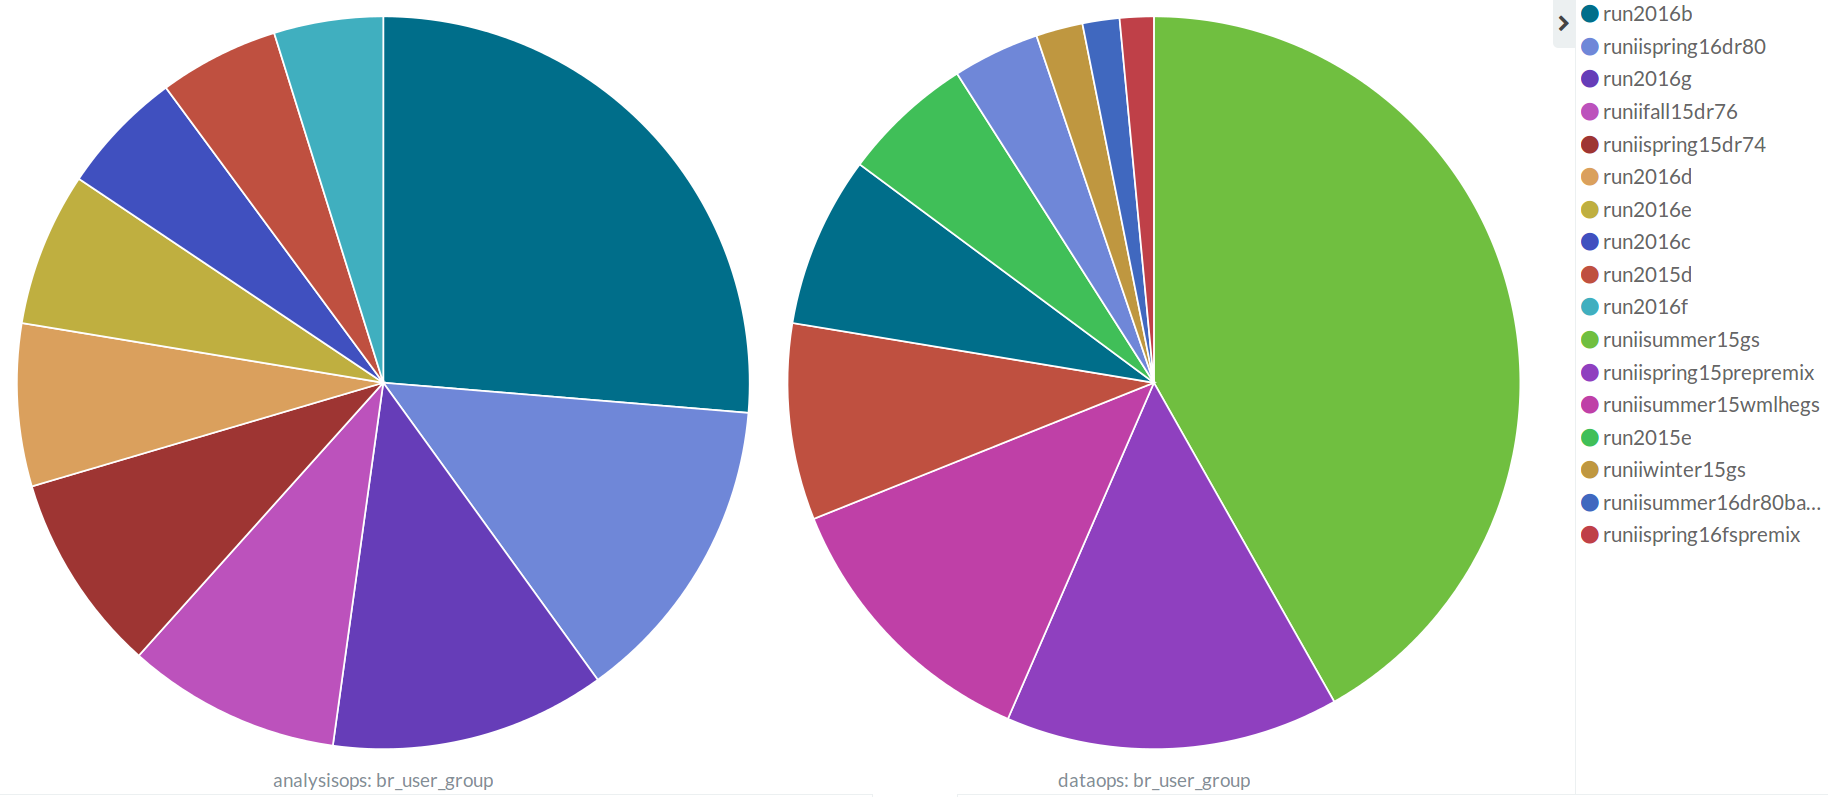
\includegraphics[width=15cm]{pie-charts}
\caption{Pie charts with kibana}
\label{fig:pie-charts}
\end{center}
\end{figure}

\subsection{Historical data analysis}

\begin{enumerate}
\item Define search that filters records which have an origin of cronjob and node kind of disk
\item Define search that filters records which have an origin of cronjob and node kind of mss
\item For each search create bar charts:
\begin{itemize}
\item Define Y axis as sum of node bytes
\item Define X axis as field now
\item Split charts by top 3 storage consuming user groups
\item Split bars by;
\begin{itemize}
\item Top 20 storage consuming acquisition eras
\item Top 20 storage consuming data tiers
\end{itemize}
\end{itemize}
\item Combine all 4 visualizations in one dashboard and save it with time "Last 7 days"
\end{enumerate}
Capture of the dashboard can be seen in \ref{fig:bar-charts}
\begin{figure}[ht]
\begin{center}
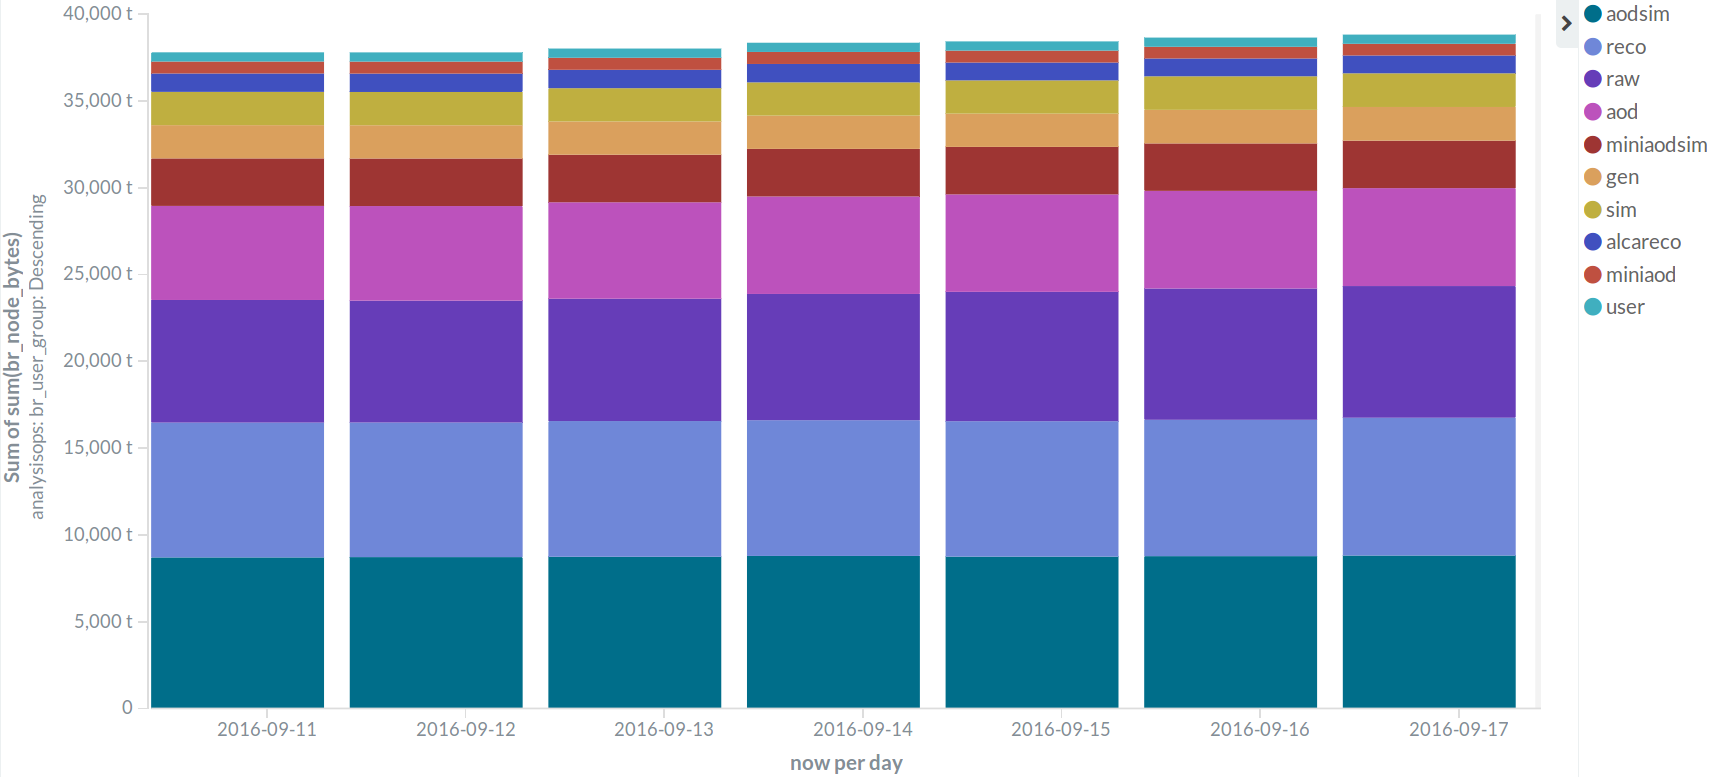
\includegraphics[width=15cm]{bar-charts}
\caption{Bar charts with kibana}
\label{fig:bar-charts}
\end{center}
\end{figure}

\section{Deployment}

Service was implemented in development environment which consisted of personl VM (where elasticsearch/kibana were installed) and analytix cluster (where spark jobs were 
submitted). Later it was moved into more accesible environment - WMArchive node. Migration process included:
\begin{itemize}
\item Creating rpm packages for the service
\item Writing deployment and management scripts\footnote{https://github.com/vkuznet/deployment/tree/master/phedexreplicamonitoring}
\item Solving kerberos authentication issues while accesing hdfs
\item Deploying elasticsearch and opening port 9200 iptables
\item Deploying kibana and opening port 5601 iptables
\item Making rpm packeges from third-party resources needed for service
\end{itemize}
Future perspecitive is to migrate service under DMWM umbrella nad use elasticsearch/kibana from central CERN IT service.
In order to use service in personal environment user should specify some environment variables (in the common usage variables will be set in manage script by programmer)
\begin{itemize}
\item SPARK{\_}CSV{\_}ASSEMBLY{\_}JAR - spark-csv package path
\item ES{\_}HADOOP{\_}JAR - elasticsearch-hadoop package path
\item PYTHONPATH - path to projects python folder. Ex.: ~/src/python
\item PBR{\_}DATA - path to external data (phedex{\_}groups.csv, phedex{\_}node{\_}kinds.csv files). Ex.: ~/data
\item PBR{\_}CONFIG - path to elasticsearch configuration (pbr.cfg). Ex.: ~/etc
\end{itemize}

\section{Conclusion}

Service really helps to analyze data by reducing its dimensions (aggregation) and visualizing it. Proposed approach has three main advantages. First of all, it is very 
efficient as it is build on top of Spark which allows distributed computing using executors memory instead of disk. Moreover, it is fully-covered. By using this service 
user can get everything from raw data in hadoop file system to visualizations and dashboards in kibana. Lastly, it is highly configurable. If a user wants to look at data 
from different perspective all he need to do is to change service parameters. By doing that he gets different agregations, different results written in hdfs and elasticsearch, 
different visualizations and dashborads in kibana. All of this without a need to change the service itself.

\end{document}
